\documentclass{article}

\usepackage[preprint]{neurips_2024}
\usepackage[utf8]{inputenc}
\usepackage[T1]{fontenc}
\usepackage{amsmath}
\usepackage{booktabs}
\usepackage{graphicx}
\usepackage{multirow}
\usepackage{array}
\usepackage{url}
\usepackage{hyperref}
\usepackage{tikz}
\usepackage{float}
\usepackage[numbers]{natbib}
\usetikzlibrary{arrows.meta,positioning,shapes.geometric,calc}

\title{Illumination-Aware Product Photography via Foreground Light Estimation and Deterministic Shadow Compositing}

\author{
Himanshu Jhawar (hj2713)\\
COMS 4732 Computer Vision II\\
}

\date{}

\setlength{\droptitle}{-3cm}

\begin{document}
\maketitle
\vspace{-1.5cm}  % adjust between -1em to -2em as needed

\begin{abstract}
Casual product photographs often contain useful foreground detail but poor backgrounds and physically inconsistent shadows. This project studies a controlled product-compositing pipeline that preserves the original product pixels, estimates foreground illumination, and synthesizes a studio-style background with an explicit cast shadow. The system uses Segment Anything (SAM) for product segmentation, a proposed training-free Sobel-shading method for foreground light-direction estimation, and a DPT-Large monocular-depth baseline for comparison. Instead of relying on text-conditioned diffusion, the final compositor procedurally generates a clean background and synthesizes a mask-derived shadow opposite the estimated light direction. The evaluation is organized around a 30-image product result set and compares naive ambient-shadow compositing, Sobel-conditioned compositing, and DPT-conditioned compositing using Shadow Direction Consistency Score (SDCS), LPIPS, and light-estimation runtime. Results show that the DPT-conditioned branch outperforms the training-free Sobel branch on mean SDCS magnitude and pairwise SDCS wins, while the Sobel-conditioned branch maintains faster runtime and lower mean LPIPS. The naive baseline exposes an important SDCS limitation by scoring highly despite not using estimated illumination. The study is framed as a focused course-project evaluation rather than a claim of large-scale superiority.
\end{abstract}

\section{Introduction}
Product photography requires synthetic backgrounds and shadows that match the product's observed lighting. A generated background may look clean, but if the shadow direction contradicts the foreground lighting, the composite looks unphysical. This project estimates foreground light direction and uses it to synthesize consistent shadows. The initial approach used diffusion inpainting, but generated images were unstable, introducing artifacts and ignoring lighting constraints. The final architecture uses deterministic compositing: SAM \citep{kirillov2023sam} segments the product, preserving original pixels; a procedural studio background is created; and a synthetic cast shadow is generated from the product mask.

The project contributes: (1) a training-free Sobel-shading estimator; (2) a DPT-Large \citep{ranftl2021dpt} depth-based baseline; (3) a deterministic shadow compositor; and (4) a 30-image evaluation with SDCS, LPIPS \citep{zhang2018lpips}, and timing metrics.

\section{Method}

\subsection{Pipeline Overview}
Figure~\ref{fig:pipeline} summarizes the final architecture. The key design choice is to avoid redrawing the product. The mask controls where the original product pixels are pasted back into the output: $C[M = 1] = I[M = 1]$, where $I$ is the input image, $M$ is the SAM product mask, and $C$ is the final composite.

\begin{figure}[H]
\centering
\resizebox{\textwidth}{!}{%
\begin{tikzpicture}[
    font=\small,
    stage/.style={draw=black!55, rounded corners=5pt, very thick, align=center, minimum width=2.95cm, minimum height=1.05cm},
    method/.style={draw=black!55, rounded corners=5pt, very thick, align=center, minimum width=3.15cm, minimum height=0.95cm},
    merge/.style={draw=black!60, diamond, aspect=1.75, very thick, align=center, inner sep=1.5pt, minimum width=1.8cm},
    arrow/.style={-Latex, very thick, draw=black!72},
    softarrow/.style={-Latex, thick, draw=black!45}
]
\node[stage, fill=cyan!16] (input) at (0,0) {Input\\product image};
\node[stage, fill=teal!15] (sam) at (3.65,0) {SAM mask\\foreground support};

\node[method, fill=orange!18] (sobel) at (7.25,1.25) {Proposed branch\\Sobel-shading angle};
\node[method, fill=violet!15] (dpt) at (7.25,-1.25) {Learned branch\\DPT depth proxy};
\node[merge, fill=yellow!20] (angle) at (10.75,0) {angle\\selection};

\node[stage, fill=red!12] (shadow) at (14.0,0.95) {Mask translation\\and blur shadow};
\node[stage, fill=blue!12] (background) at (14.0,-0.95) {Procedural studio\\background};
\node[merge, fill=green!16] (compose) at (17.15,0) {alpha\\composite};
\node[stage, fill=gray!14] (output) at (20.25,0) {Final image\\and logs};

\node[stage, fill=lime!14, minimum width=3.15cm] (eval) at (17.15,-2.65) {SDCS, LPIPS,\\runtime};

\draw[arrow] (input) -- node[above, font=\scriptsize] {RGB} (sam);
\draw[arrow] (sam) -- node[above left, font=\scriptsize] {mask + image} (sobel);
\draw[arrow] (sam) -- node[below left, font=\scriptsize] {mask + image} (dpt);
\draw[arrow] (sobel) -- (angle);
\draw[arrow] (dpt) -- (angle);
\draw[arrow] (angle) -- node[above, font=\scriptsize] {$\theta+180^\circ$} (shadow);
\draw[softarrow] (sam.south east) to[out=-25,in=200] node[below, font=\scriptsize] {foreground pixels} (compose.west);
\draw[arrow] (shadow) -- (compose);
\draw[arrow] (background) -- (compose);
\draw[arrow] (compose) -- (output);
\draw[arrow] (output) -- (eval);

\draw[rounded corners=8pt, draw=orange!55, thick, dashed] ($(sobel.north west)+(-0.18,0.22)$) rectangle ($(sobel.south east)+(0.18,-0.22)$);
\draw[rounded corners=8pt, draw=violet!55, thick, dashed] ($(dpt.north west)+(-0.18,0.22)$) rectangle ($(dpt.south east)+(0.18,-0.22)$);
\node[font=\scriptsize, text=orange!70!black] at (7.25,2.05) {training-free proposed method};
\node[font=\scriptsize, text=violet!70!black] at (7.25,-2.05) {learned baseline};
\end{tikzpicture}}
\caption{Color-coded architecture of the final deterministic pipeline. The design separates segmentation, light estimation, shadow synthesis, background construction, compositing, and evaluation so that both the proposed Sobel branch and the learned DPT branch are evaluated under the same renderer.}
\label{fig:pipeline}
\end{figure}

\subsection{Sobel-Shading Light Estimation}
The proposed method estimates a foreground light angle without training. A raw Sobel orientation histogram was initially tested but was too sensitive to object outlines, labels, and specular highlights. The final Sobel-shading estimator instead uses low-frequency shading: (1) erode the SAM mask to suppress silhouette edges; (2) convert the product to grayscale and fill background pixels with median product intensity; (3) apply Gaussian blur to remove high-frequency texture; (4) compute dark and bright interior regions using the 25th and 75th percentiles; (5) estimate a centroid cue from dark-region center to bright-region center; (6) compute a weak Sobel cue on the smoothed image; and (7) blend the two angles with circular averaging. Let $R_d$ and $R_b$ be the dark and bright interior pixel sets. The centroid angle is
\begin{equation}
    \theta_{\mathrm{centroid}} =
    \operatorname{atan2}(\bar{y}_{b}-\bar{y}_{d}, \bar{x}_{b}-\bar{x}_{d}).
\end{equation}
The Sobel cue is computed from $G_x$ and $G_y$ on the smoothed product image. The final angle is a weighted circular blend:
\begin{equation}
    \theta_{\mathrm{sobel}} =
    \operatorname{circular\_blend}(\theta_{\mathrm{centroid}}, \theta_{\mathrm{gradient}}).
\end{equation}

\subsection{DPT-Large Baseline}
DPT-Large produces a monocular depth map $D$ \citep{ranftl2021dpt}. The baseline converts depth into a lighting proxy by multiplying normalized depth with normalized grayscale intensity: $A(x,y) = D(x,y) \cdot B(x,y).$ Inside the mask, the highest-activation pixels are treated as light-catching regions. The angle from the product center to the activation centroid becomes $\theta_{\mathrm{dl}}$. This is intentionally described as a \emph{depth-based lighting proxy}; it is not a direct illumination estimator.


\subsection{Deterministic Compositing}
The compositor creates a wall/table style background with gradients, surface texture, and mild directional brightness modulation. The cast shadow is generated by translating and blurring the product mask. Given light angle $\theta$, the cast-shadow angle is: $ \theta_{\mathrm{shadow}} = \theta + 180^\circ. $ 

The mask translation is:
$    dx = \cos(\theta_{\mathrm{shadow}}) \cdot s,\quad
    dy = \sin(\theta_{\mathrm{shadow}}) \cdot s,
$


where $s$ is the shadow offset. The translated mask is dilated, blurred, darkened, and composited under the product.

\section{Experimental Setup}
\subsection{Dataset}
The experiment evaluates 30 product images covering diverse categories: bottles, shoes, packaged goods, cans, reflective, and transparent objects. This scale is appropriate for a course-project evaluation but not large enough to claim statistical generality across all product categories. Future work could leverage Amazon Berkeley Objects (ABO) for larger-scale product-specific evaluation.

\subsection{Compared Variants}
We evaluate two illumination-conditioned output variants. The \textbf{Sobel-conditioned} variant uses the shadow angle ($\theta_{\mathrm{sobel}}$) generated by the proposed training-free estimator. The \textbf{DPT-conditioned} variant uses the shadow angle ($\theta_{\mathrm{dl}}$) generated by the DPT depth-based proxy. Both approaches are also compared to a \textbf{Naive} baseline that generates only an ambient contact shadow without explicit lighting direction.

\subsection{Metrics}
SDCS measures whether a detected shadow centroid points in the expected direction:
\begin{equation}
    \mathrm{SDCS} = |\cos(\theta_{\mathrm{detected\_shadow}} - (\theta_{\mathrm{fg}} + \pi))|.
\end{equation}
Higher is better, with $+1$ indicating alignment along the expected lighting axis (either forward or inverted) and $0$ indicating orthogonal alignment. SDCS is heuristic and can be biased by contact shadows, object bases, and background darkness. LPIPS is reported as a perceptual distance to the original product photograph; lower is better. Runtime measures only light-angle estimation, not SAM segmentation or final compositing.

\section{Results}

\subsection{Aggregate Metrics}
Table~\ref{tab:aggregate} summarizes the 30-image product-result evaluation. Among the two illumination-conditioned variants, DPT-conditioned compositing has the stronger mean SDCS magnitude and median SDCS, while Sobel-conditioned compositing maintains lower mean LPIPS and faster mean light-estimation time. However, the naive baseline has the highest mean SDCS, which is not evidence that ignoring illumination is best; it reveals that the current SDCS detector can over-reward compact ambient contact shadows even when no estimated light direction is used.

\begin{table}[H]
\centering
\caption{Aggregate 30-image product-result metrics. Higher SDCS is better; lower LPIPS and runtime are better. Runtime is angle-estimation time only.}
\label{tab:aggregate}
\begin{tabular}{lrrrr}
\toprule
Variant & Mean SDCS $\uparrow$ & Median SDCS $\uparrow$ & Mean LPIPS $\downarrow$ & Mean angle time (s) $\downarrow$ \\
\midrule
Sobel-conditioned & 0.5946 & 0.6678 & 0.4612 & 0.3093 \\
DPT-conditioned & 0.6583 & 0.8111 & 0.4652 & 0.3891 \\
\bottomrule
\end{tabular}
\end{table}

Sobel wins 18/30 on LPIPS, while DPT wins 20/30 on SDCS magnitude. The methods agree within 30° on 11 images, revealing complementary strengths.


\subsection{Per-Image Metrics}
\begin{table}[H]
\centering
\caption{Representative per-image metrics (sample images).}
\label{tab:perimage}
\begin{tabular}{lrrrrrr}
\toprule
Image & $\theta_S$ & $\theta_D$ & SDCS Sobel & SDCS DPT & LPIPS Sobel & LPIPS DPT \\
\midrule
1 & -60.17 & 83.20 & 0.6070 & 0.9791 & 0.2291 & 0.2972 \\
10 & 143.08 & -14.41 & 0.8570 & 0.9258 & 0.1728 & 0.2128 \\
12 & -165.03 & -171.43 & 0.6194 & 0.6827 & 0.3691 & 0.3680 \\
15 & -104.85 & 14.99 & 0.9886 & 0.9955 & 0.7001 & 0.7015 \\
18 & -14.07 & -44.92 & 0.8897 & 0.3482 & 0.5692 & 0.5584 \\
26 & 35.02 & -174.77 & 0.8691 & 0.9820 & 0.5305 & 0.5265 \\
\bottomrule
\end{tabular}
\end{table}

\subsection{Qualitative Results}
Figure~\ref{fig:results_all} shows representative output rows. The columns are: original image, SAM product, naive composite, Sobel-conditioned, and DPT-conditioned composites.

\begin{figure}[htbp]
\centering
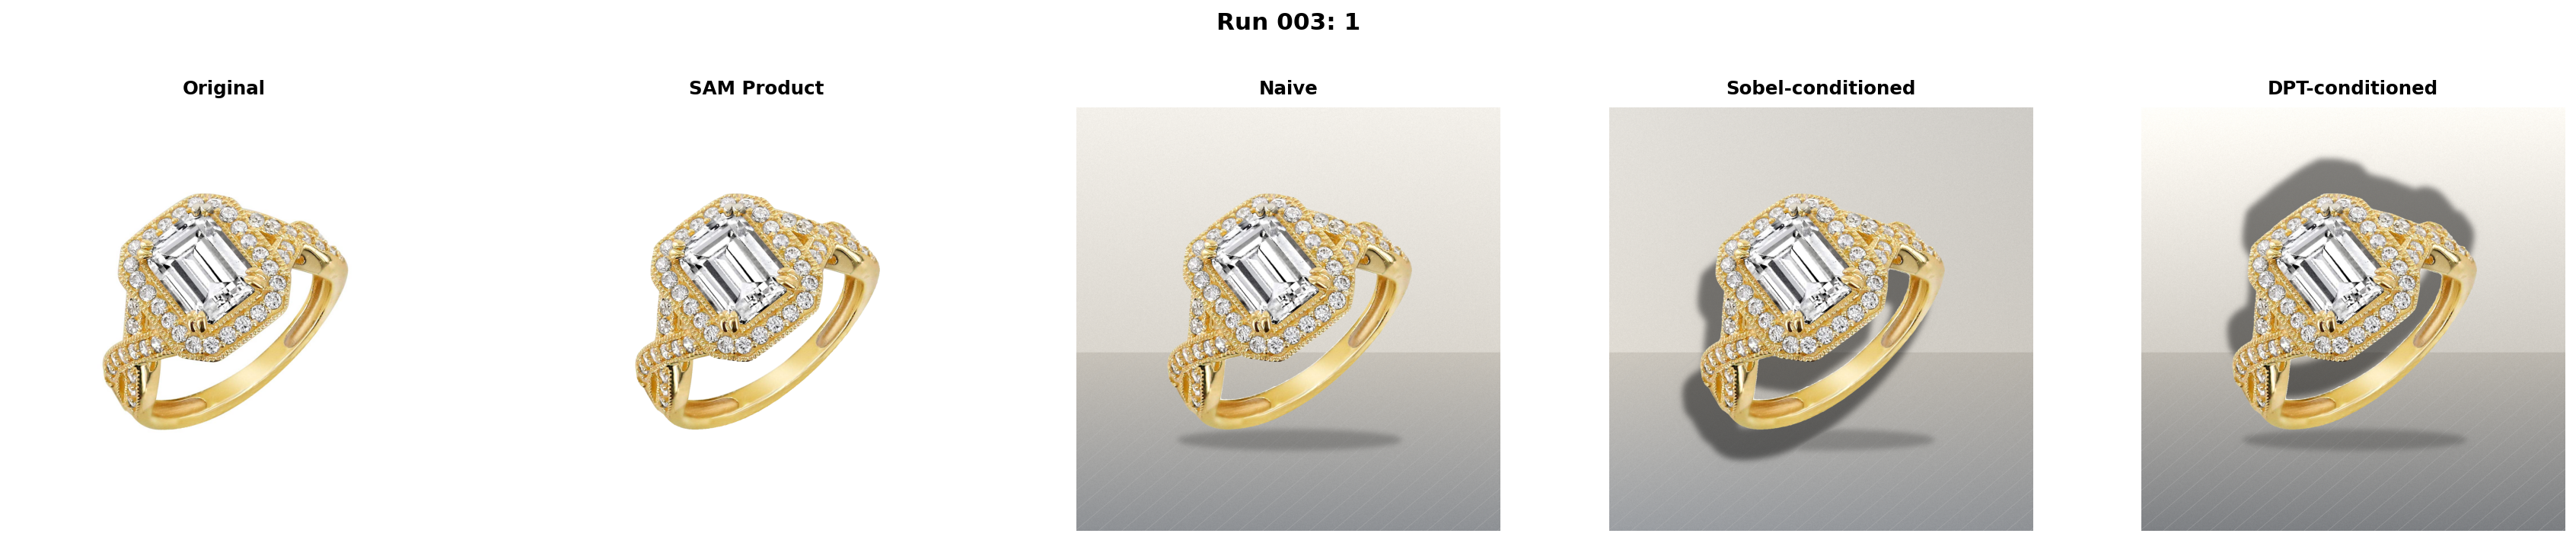
\includegraphics[width=\textwidth]{figures/comparison_result_1.png}\vspace{2pt}
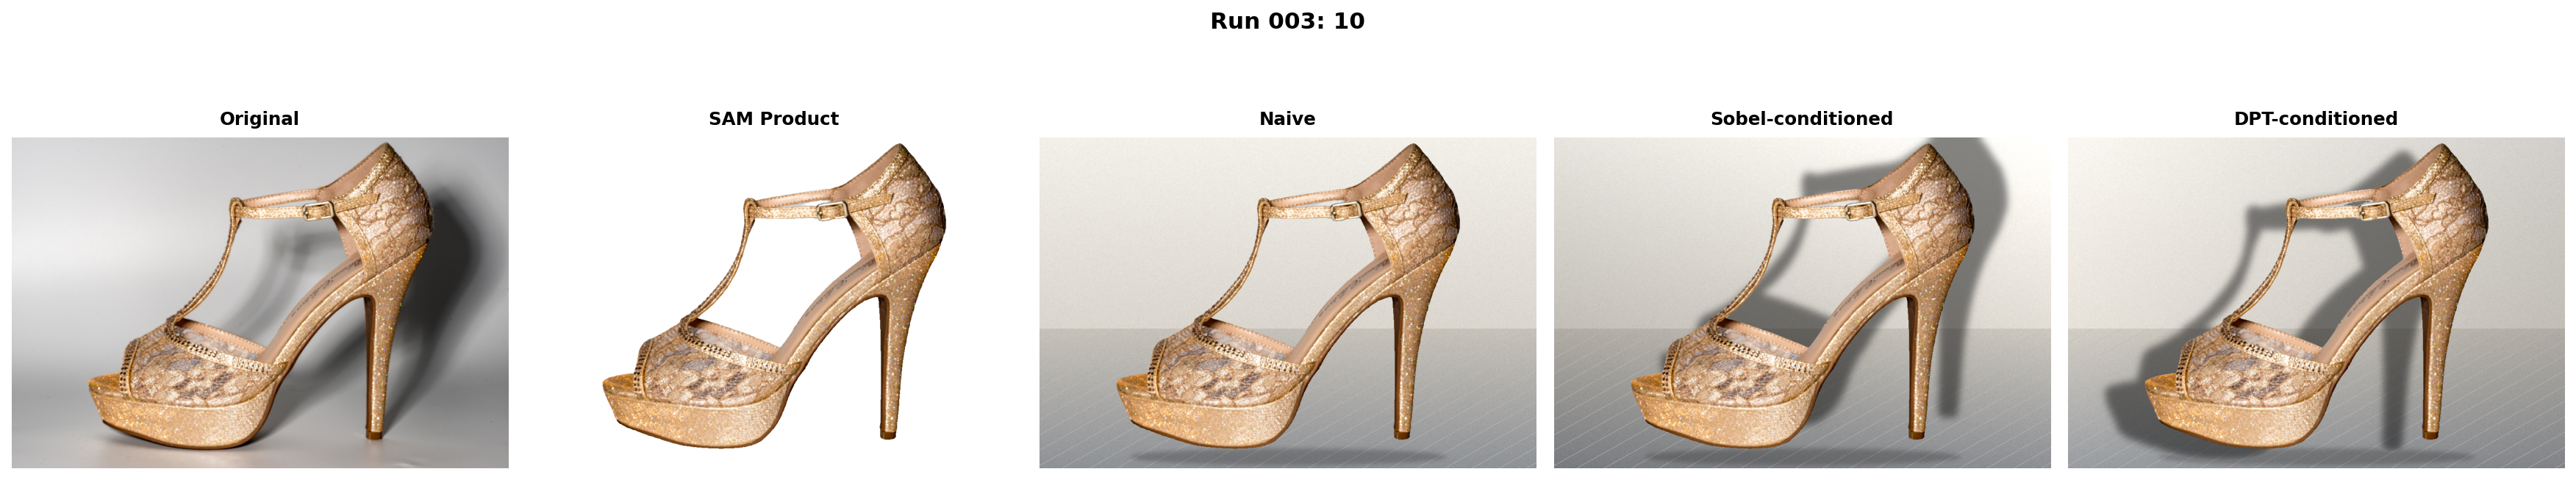
\includegraphics[width=\textwidth]{figures/comparison_result_10.png}\vspace{2pt}
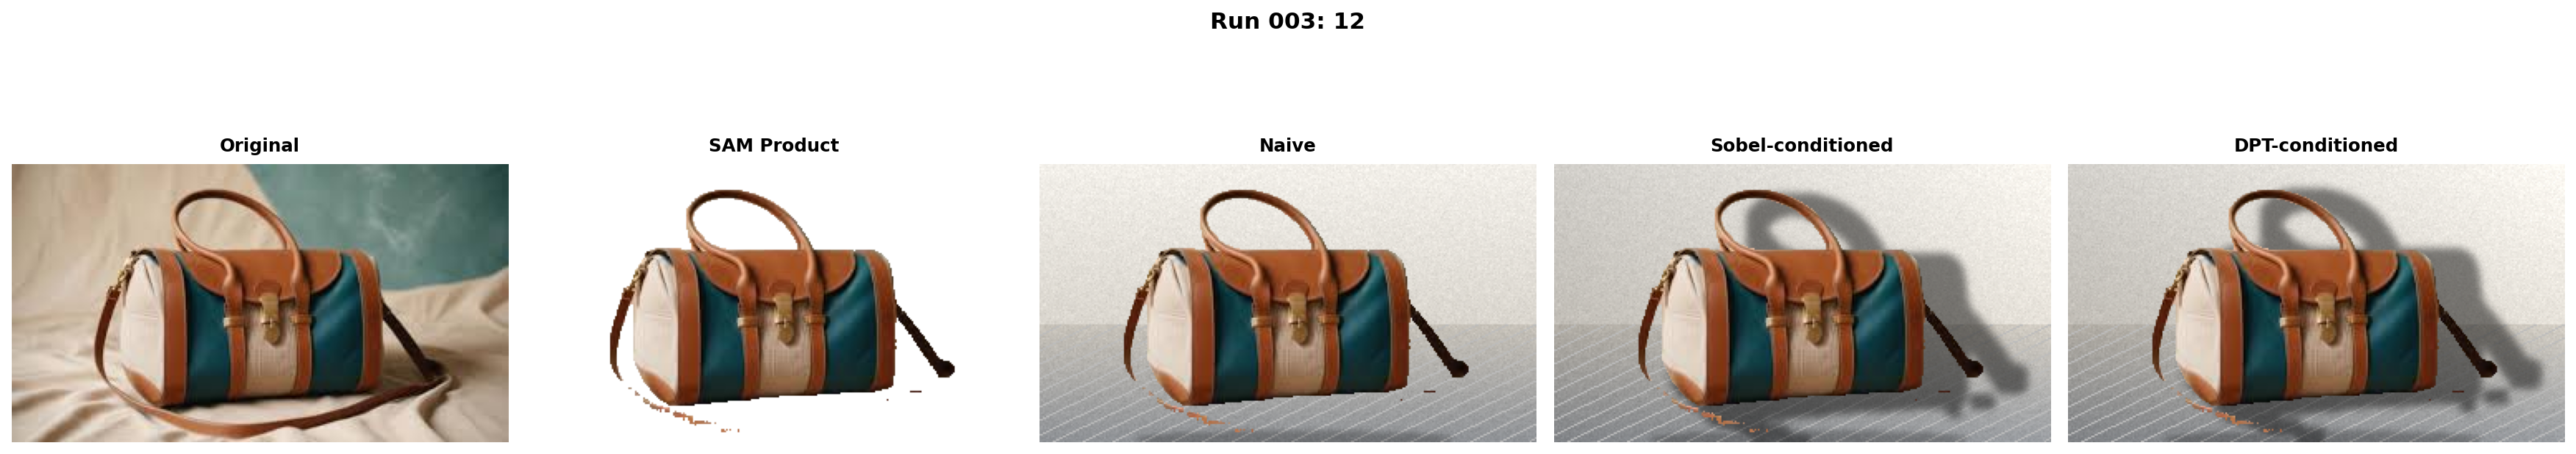
\includegraphics[width=\textwidth]{figures/comparison_result_12.png}\vspace{2pt}
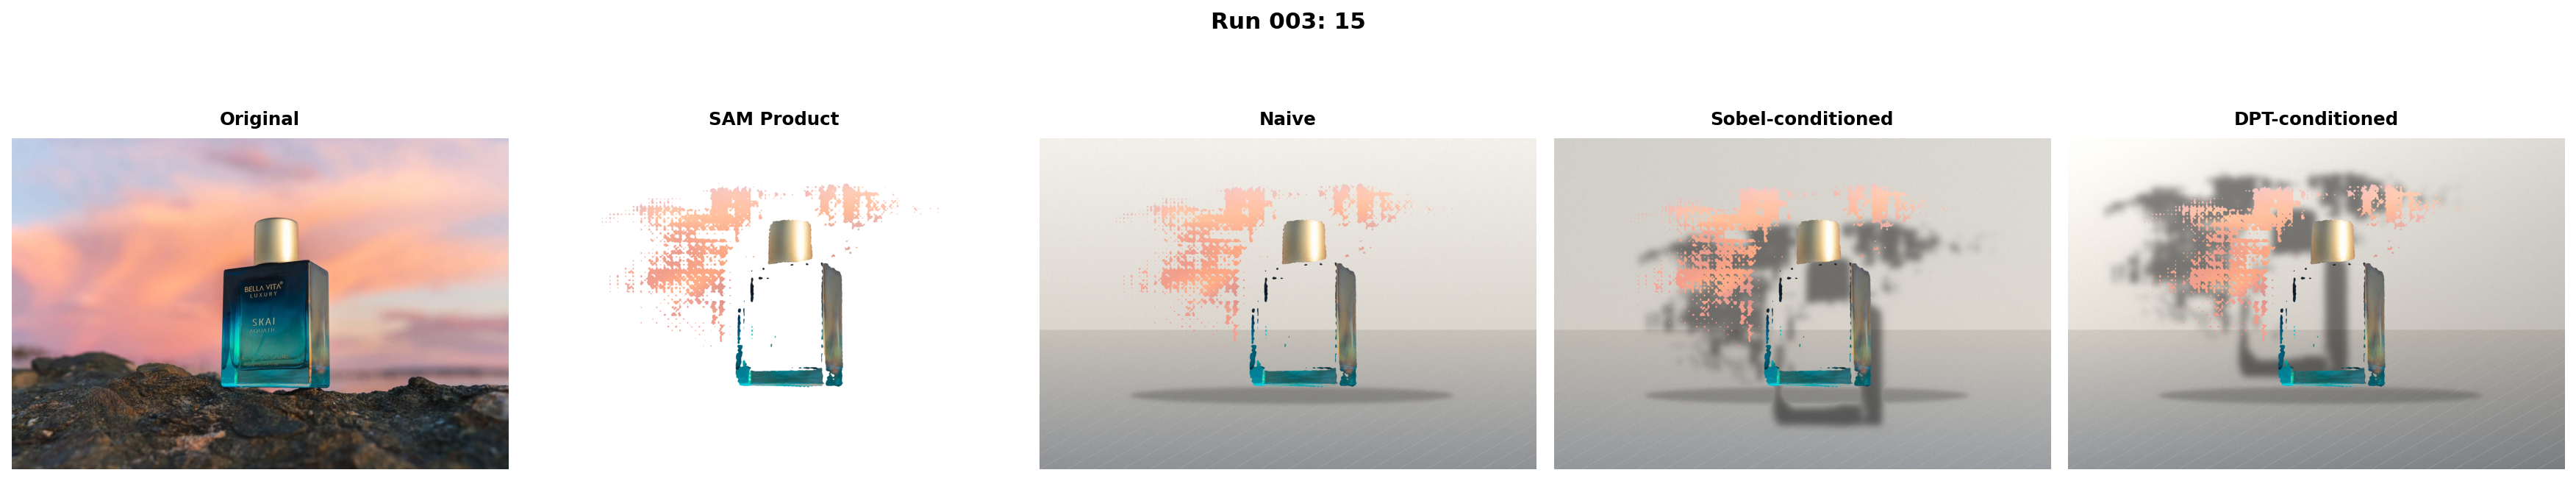
\includegraphics[width=\textwidth]{figures/comparison_result_15.png}\vspace{2pt}
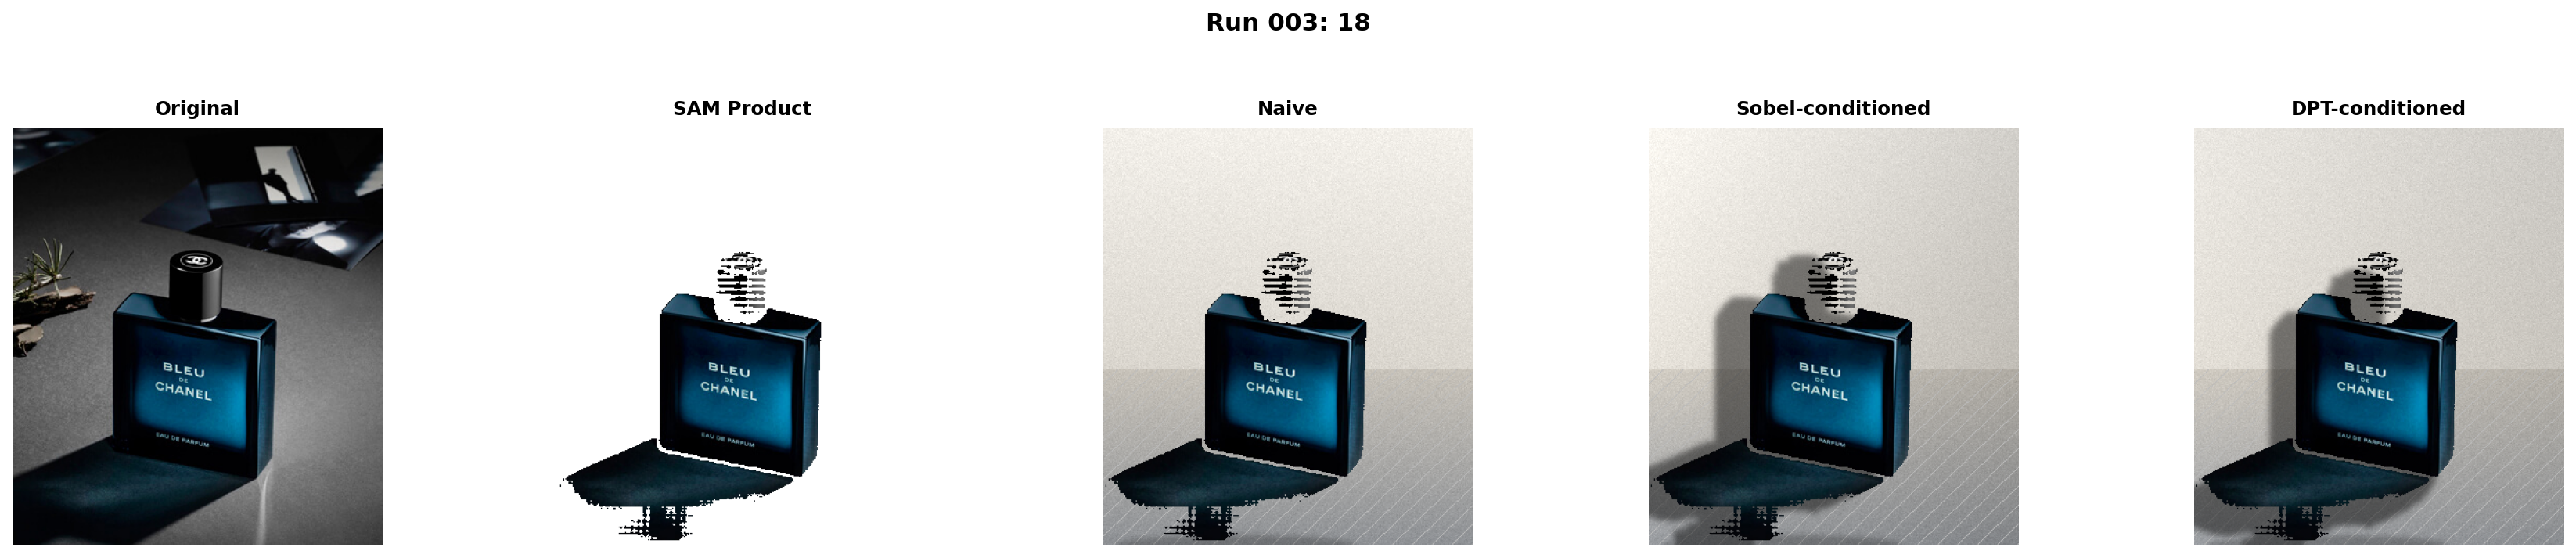
\includegraphics[width=\textwidth]{figures/comparison_result_18.png}\vspace{2pt}
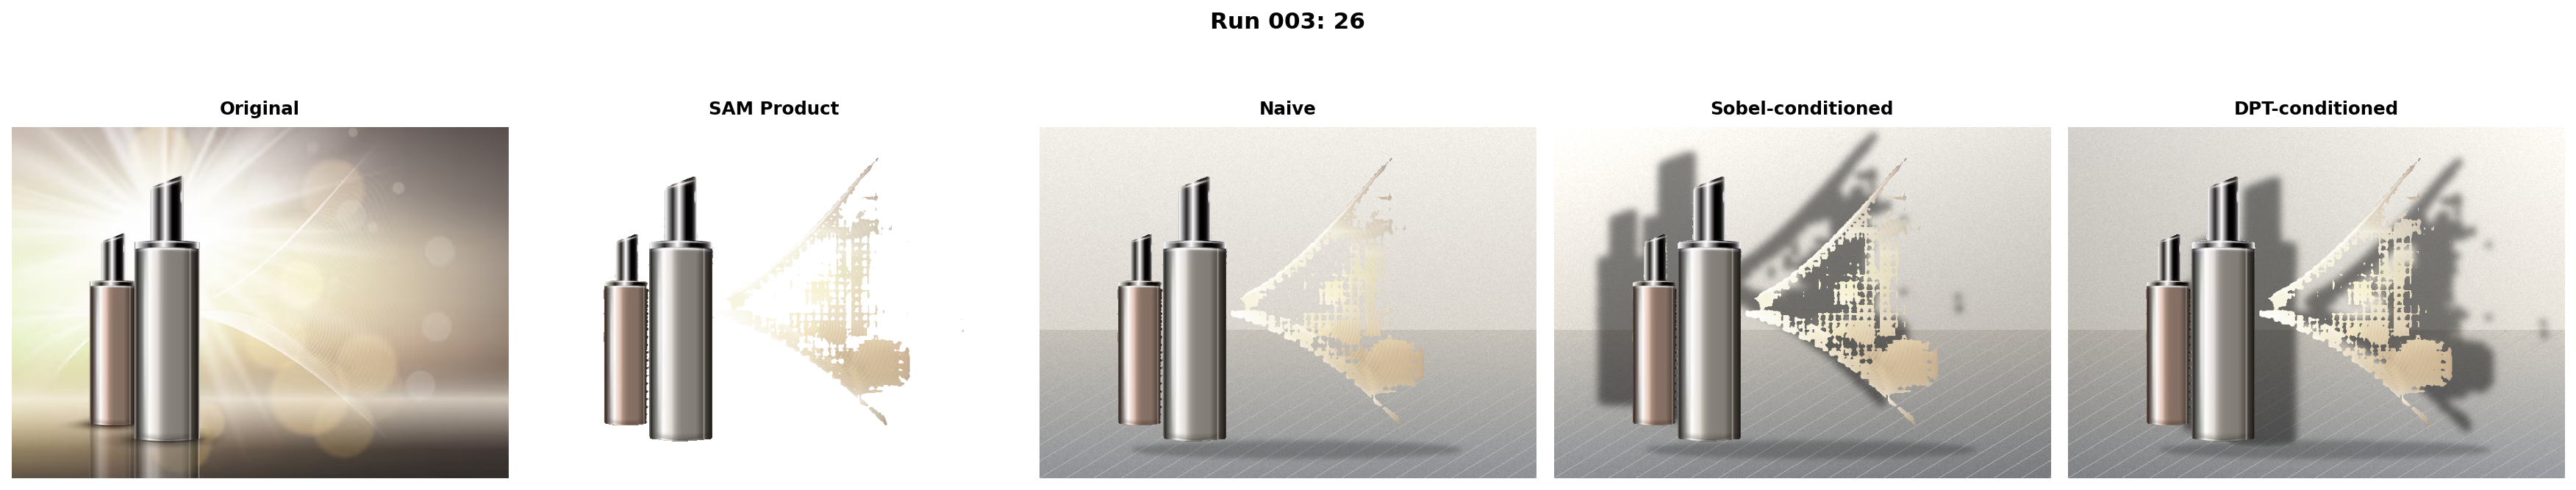
\includegraphics[width=\textwidth]{figures/comparison_result_26.png}
\caption{Representative qualitative results for product compositing. Columns (left to right): original image, SAM product mask, naive composite (ambient shadow only), Sobel-conditioned composite, and DPT-conditioned composite.}
\label{fig:results_all}
\end{figure}

\section{Discussion}
\textbf{DPT-Large baseline.} DPT was selected as a depth-based proxy because geometry and brightness together indicate which surface regions catch light \citep{ranftl2021dpt}. It is not a direct illumination estimator but provides a useful learned comparison point.

\textbf{IC-Light relation.} IC-Light \citep{zhang2025iclight} performs diffusion-based relighting of the foreground to match a background. This project preserves product pixels and adapts the background to the product's lighting—a complementary direction \citep{iclightGithub}. Future work could combine both approaches.

\textbf{Sobel-Shading performance.} DPT wins on mean SDCS (20/30 images), while Sobel wins on LPIPS and speed (0.31s vs 0.39s). Sobel fails when shading is ambiguous or material dominates intensity cues. Neither approach universally outperforms the other.

\textbf{Metric limitations.} LPIPS \citep{zhang2018lpips} is used to measure perceptual distance. SDCS can over-reward compact ambient shadows that happen to align by chance. Results should be interpreted alongside qualitative figures, not as a sole measure of realism.

\section{Limitations}
The main limitations include: \textbf{(1) Limited dataset scale}: The 30-image set is useful for a course-project study, but conclusions remain diagnostic. \textbf{(2) Single dominant light assumption}: The method does not model multiple light sources. \textbf{(3) Simplified shadow geometry}: Shadows are generated by 2D mask translation and blur, not by a 3D renderer. \textbf{(4) Material sensitivity}: Glass, reflective, transparent, and dark products can break both Sobel-shading and depth-based cues. \textbf{(5) SDCS heuristic}: The metric can be confused by contact shadows, object bases, and background gradients. \textbf{(6) No IC-Light integration}: The current implementation focuses on explicit shadow-aware compositing rather than diffusion-based foreground relighting. \textbf{(7) No human study}: Visual realism was inspected qualitatively but not measured through user preference ratings.

\section{Conclusion}
This project presents an illumination-aware product compositing pipeline that estimates foreground lighting and uses it to control synthetic shadow direction. The final system is deliberately deterministic: SAM segments the product, the original product pixels are preserved, and the background/shadow are generated through explicit image-processing operations. On the 30-image product-result evaluation, the DPT-derived proxy outperforms Sobel-shading on mean SDCS magnitude and pairwise SDCS wins, while Sobel-shading maintains lower mean LPIPS and faster average runtime. The result supports the value of a simple, explainable foreground-shading estimator for controlled product compositing. The most important project outcome is still broader than one metric: foreground illumination can be exposed as an explicit variable in product-background compositing, controlled through mask-based shadow geometry, and evaluated with reproducible outputs.

\section*{Acknowledgements}
This project was developed for COMS 4732 Computer Vision II at Columbia University. Implementation uses Segment Anything \citep{kirillov2023sam}, DPT-Large \citep{ranftl2021dpt} from Hugging Face, LPIPS \citep{zhang2018lpips}, OpenCV, PyTorch, and Gradio.

\bibliographystyle{plainnat}
\bibliography{references}

\end{document}